\documentclass{standalone}

\usepackage[OT1]{fontenc}
\usepackage[onlymath]{sansmathfonts}
\usepackage{tikz}

\begin{document}
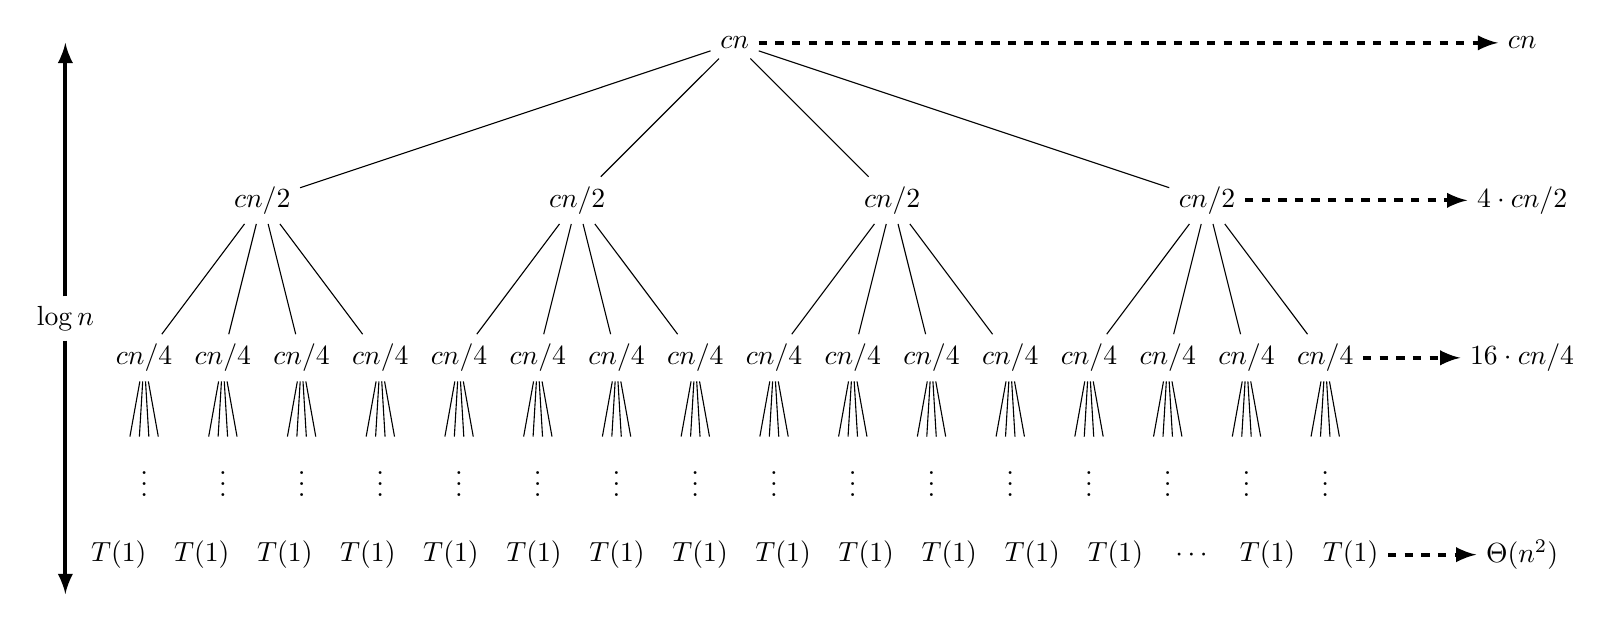
\begin{tikzpicture}
    % Root
        \node (r) at (0,0) {$cn$};

        % One layer of 4 children
        \node (c1) at (-6,-2) {$cn/2$};
        \node (c2) at (-2,-2) {$cn/2$};
        \node (c3) at ( 2,-2) {$cn/2$};
        \node (c4) at ( 6,-2) {$cn/2$};

        % Second layer
        \node (c11) at (-7.5,-4) {$cn/4$};
        \node (c12) at (-6.5,-4) {$cn/4$};
        \node (c13) at (-5.5,-4) {$cn/4$};
        \node (c14) at (-4.5,-4) {$cn/4$};
        \node (c21) at (-3.5,-4) {$cn/4$};
        \node (c22) at (-2.5,-4) {$cn/4$};
        \node (c23) at (-1.5,-4) {$cn/4$};
        \node (c24) at (-0.5,-4) {$cn/4$};
        \node (c31) at ( 0.5,-4) {$cn/4$};
        \node (c32) at ( 1.5,-4) {$cn/4$};
        \node (c33) at ( 2.5,-4) {$cn/4$};
        \node (c34) at ( 3.5,-4) {$cn/4$};
        \node (c41) at ( 4.5,-4) {$cn/4$};
        \node (c42) at ( 5.5,-4) {$cn/4$};
        \node (c43) at ( 6.5,-4) {$cn/4$};
        \node (c44) at ( 7.5,-4) {$cn/4$};

        % dots
        \node (dots1) at (-7.5,-5.5) {$\vdots$};
        \node (dots2) at (-6.5,-5.5) {$\vdots$};
        \node (dots3) at (-5.5,-5.5) {$\vdots$};
        \node (dots4) at (-4.5,-5.5) {$\vdots$};
        \node (dots5) at (-3.5,-5.5) {$\vdots$};
        \node (dots6) at (-2.5,-5.5) {$\vdots$};
        \node (dots7) at (-1.5,-5.5) {$\vdots$};
        \node (dots8) at (-0.5,-5.5) {$\vdots$};
        \node (dots9) at ( 0.5,-5.5) {$\vdots$};
        \node (dots10) at ( 1.5,-5.5) {$\vdots$};
        \node (dots11) at ( 2.5,-5.5) {$\vdots$};
        \node (dots12) at ( 3.5,-5.5) {$\vdots$};
        \node (dots13) at ( 4.5,-5.5) {$\vdots$};
        \node (dots14) at ( 5.5,-5.5) {$\vdots$};
        \node (dots15) at ( 6.5,-5.5) {$\vdots$};
        \node (dots16) at ( 7.5,-5.5) {$\vdots$};

        % T(1) leaves
        \node (leaf1) at (0, -6.5) {$T(1)\quad T(1)\quad T(1)\quad T(1)\quad T(1)\quad T(1)\quad T(1)\quad T(1)\quad T(1)\quad T(1)\quad T(1)\quad T(1)\quad T(1)\quad\cdots\quad T(1)\quad T(1)$};

        % Edges (straight lines)
        \draw (r) -- (c1);
            \draw (c1) -- (c11);
                \draw (c11) -- (-7.68, -5);
                \draw (c11) -- (-7.56, -5);
                \draw (c11) -- (-7.44, -5);
                \draw (c11) -- (-7.32, -5);
            \draw (c1) -- (c12);
                \draw (c12) -- (-6.68, -5);
                \draw (c12) -- (-6.56, -5);
                \draw (c12) -- (-6.44, -5);
                \draw (c12) -- (-6.32, -5);
            \draw (c1) -- (c13);
                \draw (c13) -- (-5.68, -5);
                \draw (c13) -- (-5.56, -5);
                \draw (c13) -- (-5.44, -5);
                \draw (c13) -- (-5.32, -5);
            \draw (c1) -- (c14);
                \draw (c14) -- (-4.68, -5);
                \draw (c14) -- (-4.56, -5);
                \draw (c14) -- (-4.44, -5);
                \draw (c14) -- (-4.32, -5);
        \draw (r) -- (c2);
            \draw (c2) -- (c21);
                \draw (c21) -- (-3.68, -5);
                \draw (c21) -- (-3.56, -5);
                \draw (c21) -- (-3.44, -5);
                \draw (c21) -- (-3.32, -5);
            \draw (c2) -- (c22);
                \draw (c22) -- (-2.68, -5);
                \draw (c22) -- (-2.56, -5);
                \draw (c22) -- (-2.44, -5);
                \draw (c22) -- (-2.32, -5);
            \draw (c2) -- (c23);
                \draw (c23) -- (-1.68, -5);
                \draw (c23) -- (-1.56, -5);
                \draw (c23) -- (-1.44, -5);
                \draw (c23) -- (-1.32, -5);
            \draw (c2) -- (c24);
                \draw (c24) -- (-0.68, -5);
                \draw (c24) -- (-0.56, -5);
                \draw (c24) -- (-0.44, -5);
                \draw (c24) -- (-0.32, -5);
        \draw (r) -- (c3);
            \draw (c3) -- (c31);
                \draw (c31) -- (0.32, -5);
                \draw (c31) -- (0.44, -5);
                \draw (c31) -- (0.56, -5);
                \draw (c31) -- (0.68, -5);
            \draw (c3) -- (c32);
                \draw (c32) -- (1.32, -5);
                \draw (c32) -- (1.44, -5);
                \draw (c32) -- (1.56, -5);
                \draw (c32) -- (1.68, -5);
            \draw (c3) -- (c33);
                \draw (c33) -- (2.32, -5);
                \draw (c33) -- (2.44, -5);
                \draw (c33) -- (2.56, -5);
                \draw (c33) -- (2.68, -5);
            \draw (c3) -- (c34);
                \draw (c34) -- (3.32, -5);
                \draw (c34) -- (3.44, -5);
                \draw (c34) -- (3.56, -5);
                \draw (c34) -- (3.68, -5);
        \draw (r) -- (c4);
            \draw (c4) -- (c41);
                \draw (c41) -- (4.32, -5);
                \draw (c41) -- (4.44, -5);
                \draw (c41) -- (4.56, -5);
                \draw (c41) -- (4.68, -5);
            \draw (c4) -- (c42);
                \draw (c42) -- (5.32, -5);
                \draw (c42) -- (5.44, -5);
                \draw (c42) -- (5.56, -5);
                \draw (c42) -- (5.68, -5);
            \draw (c4) -- (c43);
                \draw (c43) -- (6.32, -5);
                \draw (c43) -- (6.44, -5);
                \draw (c43) -- (6.56, -5);
                \draw (c43) -- (6.68, -5);
            \draw (c4) -- (c44);
                \draw (c44) -- (7.32, -5);
                \draw (c44) -- (7.44, -5);
                \draw (c44) -- (7.56, -5);
                \draw (c44) -- (7.68, -5);

        % Right column
        \node (l1_sum) at (10, 0) {\(cn\)};
        \node (l2_sum) at (10, -2) {\(4 \cdot cn/2\)};
        \node (l3_sum) at (10, -4) {\(16 \cdot cn/4\)};
        \node (base_sum) at (10, -6.5) {$\Theta(n^2)$};

        % arrows to right column
        \draw[->, thick, dashed, >=latex, line width=1.5pt] (r) -- (l1_sum);
        \draw[->, thick, dashed, >=latex, line width=1.5pt] (c4) -- (l2_sum);
        \draw[->, thick, dashed, >=latex, line width=1.5pt] (c44) -- (l3_sum);
        \draw[->, thick, dashed, >=latex, line width=1.5pt] (leaf1) -- (base_sum);

        % tree height
        \node (h) at (-8.5, -3.5) {$\log n$};
        \draw[->, thick, >=latex, line width=1.5pt] (h) -- (-8.5, 0);
        \draw[->, thick, >=latex, line width=1.5pt] (h) -- (-8.5, -7);
\end{tikzpicture}
\end{document}